\documentclass[12pt, a4paper]{article}

% ---------- Fonts (Times New Roman) ----------
\usepackage{newtxtext}      % Times New Roman for body text
\usepackage{newtxmath}      % Matching math font (Times-style)

% ---------- Encoding ----------
\usepackage[utf8]{inputenc}
\usepackage[T1]{fontenc}
\usepackage[english]{babel}

% ---------- Layout ----------
\usepackage{geometry}
\geometry{top=2.5cm, bottom=2.5cm, left=3cm, right=2.5cm}
\usepackage{setspace}
\onehalfspacing

% ---------- Math ----------
\usepackage{amsmath, amssymb, amsthm}
\usepackage{bm}

% ---------- Graphics & Tables ----------
\usepackage{graphicx}
\usepackage{float}
\usepackage{booktabs}
\usepackage{caption}
\captionsetup{font=small, labelfont=bf}
\usepackage{subcaption}

% ---------- Code Listings ----------
\usepackage{listings}
\usepackage{xcolor}
\lstset{
    basicstyle=\ttfamily\small,
    keywordstyle=\color{blue},
    commentstyle=\color{gray!80!black},
    stringstyle=\color{red!70!black},
    breaklines=true,
    frame=single,
    numbers=left,
    numberstyle=\tiny,
    language=Python,
    showstringspaces=false
}



% ---------- Links ----------
\usepackage[hidelinks]{hyperref}
\usepackage{cleveref}

% ---------- Harvard Bibliography (BibLaTeX) ----------
\usepackage[style=ieee,backend=biber,sorting=nyt,maxbibnames=99,giveninits=true,]{biblatex}
\addbibresource{includes/references.bib}

% ============================================================
\begin{document}

% ---------- Cover Page ----------
\thispagestyle{empty}
\begin{titlepage}
{
    \centering
    \normalsize

    \vspace*{-3cm}

    
\includegraphics[width=1.3in]{images/tu_logo.png}\\[0.5em]
    \textbf{TRIBHUVAN UNIVERSITY}\\
    \textbf{INSTITUTE OF ENGINEERING}\\
    \textbf{THAPATHALI CAMPUS}
    \\[1.5cm]

    \textbf{Report NO.: }
    \\[1.5cm]

    \vspace*{-1cm}
    {\bf \MakeUppercase{Causal Self-Attention \& Decoder-Only Transformer: A GPT-Style Language Model from Scratch}}\\[0.75cm]
    \textbf{for the partial fulfillment of the coursework of the  practical  approach of deep learning}
    
    \vspace{5cm}

 % ---------- Two-Column: Submitted By | Submitted To ----------
\noindent
\begin{minipage}[t]{0.50\textwidth}
    \begin{flushleft}
        \textbf{Submitted By:}\\[0.5em]
        \textbf{\MakeUppercase{Raju Karki}}\\[0.4em]
        Roll No.: THA081MSISE012\\[0.4em]
        Date: \today
    \end{flushleft}
\end{minipage}%
\begin{minipage}[t]{0.50\textwidth}
    \begin{flushleft}
        
    
        \textbf{Submitted To:}\\[0.3em]
        \textbf{Asst. Prof. Himalaya kaKshapati}\\[0.3em]
        Department of Electronics and Computer Engineering\\[0.3em]
        Kathmandu University
  \end{flushleft}
\end{minipage}

\vfill

    \textbf{\today}\par
}
\end{titlepage}

% ---------- Front Matter ----------
\newpage
\pagenumbering{roman}
\setcounter{page}{1}

\begin{abstract}
\noindent
The architecture combines learnable token embeddings with sinusoidal 
positional encodings, a manually implemented causal multi-head self-attention 
module, pre-LayerNorm Transformer blocks with GELU-activated feed-forward 
networks, and residual connections throughout. Training employs mixed-precision 
(fp16/bf16) computation via \texttt{torch.cuda.amp.autocast} and 
\texttt{GradScaler}, a cosine annealing learning-rate schedule with a linear 
warmup phase, and the AdamW optimiser with weight decay applied only to 
2D weight matrices, excluding LayerNorm gains and bias vectors. Autoregressive 
inference supports greedy decoding, temperature scaling, and top-$k$ sampling. 
Experiments on a character-level Shakespeare corpus demonstrate stable training 
dynamics, coherent generation, and a clear trade-off between sample diversity 
and coherence as temperature and $k$ are varied. The report concludes with a 
discussion of design choices, computational considerations, and directions 
for future extension.

\vspace{0.5em}
\noindent\textbf{Keywords:} Decoder-only Transformer, Causal Self-Attention, 
Pre-LayerNorm, Mixed Precision, AdamW, Cosine Annealing, Autoregressive 
Generation, Top-$k$ Sampling.
\end{abstract}
\newpage
\section*{Acknowledgement}
\addcontentsline{toc}{section}{Acknowledgement}

I sincerely thank \textbf{Asst.\ Prof.\ Himalaya Kakshapati}, 
Department of Electronics and Computer Engineering, Thapathali Campus, 
Institute of Engineering, Tribhuvan University, for his guidance and 
continuous support throughout this assignment. This work was carried out 
as part of the coursework for the \textit{Practical Approach of Deep 
Learning} course taught by him. His lectures on attention mechanisms, 
autoregressive modelling, and modern optimisation techniques formed the 
conceptual foundation for this project, and his feedback during the 
implementation phase clarified several subtle points, particularly around 
causal masking, mixed-precision training, and parameter-group weight decay.

\noindent I am also grateful to the Department of Electronics and Computer 
Engineering, Thapathali Campus, Institute of Engineering, Tribhuvan 
University, for providing the academic environment and computational 
resources needed to complete this work.

\noindent Finally, I thank my classmates for the many discussions on Transformer 
architectures, mixed-precision optimisation, and sampling strategies that 
helped me reason through design choices during the implementation. Their 
willingness to compare notes on loss curves, gradient behaviour, and 
debugging strategies made the project significantly smoother than it would 
have been otherwise.

\vspace{0.25cm}
\noindent
\textbf{Raju Karki}\\
Roll No.: THA081MSISE012

\newpage
\tableofcontents
\newpage
\listoffigures
\newpage
\listoftables



% ---------- Main Matter ----------
\newpage
\pagenumbering{arabic}
\setcounter{page}{1}

\section{Introduction}
\label{sec:intro}

Autoregressive language models built on the Transformer architecture have
become the dominant paradigm in natural language processing, powering
systems such as GPT, LLaMA, and PaLM
\parencite{vaswani2017attention, radford2019language, brown2020language}.
The core innovation of the Transformer is the self-attention mechanism,
which allows each token to attend to every other token in the sequence
while remaining fully parallelisable across the time dimension. In a
\emph{decoder-only} configuration, attention is constrained by a causal
mask so that position $t$ can only attend to positions $\leq t$, making
the model suitable for autoregressive generation where each token is
predicted conditioned on the entire prefix before it.

\noindent The motivation for this work is that implementing a Transformer from
scratch without relying on high-level abstractions such as
\texttt{nn.TransformerDecoder} or \texttt{nn.Multihead} -{Atention} forces
an intimate understanding of the underlying tensor operations, gradient
flow, and numerical stability concerns. These details are precisely the
ones that distinguish a model that merely trains from one that trains
efficiently and generalises well \parencite{karpathy2023nanogpt}. Framed
differently: most practitioners can call a Transformer library function
and get a working model. Far fewer can explain why the causal mask is
necessary for correctness, why the square-root scaling in the attention
formula prevents softmax saturation, or why decaying a LayerNorm gain
hurts. This report is an attempt to close that gap in my own
understanding by building the entire stack from primitives.

\subsection{Problem Statement}
While high-level libraries make it easy to instantiate a Transformer,
they abstract away the causal masking logic, mixed-precision numerics,
and parameter-group weight decay that are essential for competitive
performance. The problem addressed in this report is to implement a
complete, production-style decoder-only Transformer using only PyTorch
tensor primitives, train it on a real text corpus, and verify that its
training and generation behaviour matches the theoretical expectations
set out in the literature.

\subsection{Objectives}
The specific objectives of this assignment are:
\begin{enumerate}
    \item To implement token and sinusoidal positional embeddings from
          scratch.
    \item To implement causal multi-head self-attention manually, including
          the scaled dot-product formulation and the lower-triangular mask.
    \item To build a Pre-LN Transformer block with residual connections and
          a GELU feed-forward network.
    \item To implement mixed-precision training using
          \texttt{torch.autocast} together with a
          \texttt{GradScaler} (active under fp16, disabled under bf16).
    \item To implement a cosine-annealing learning-rate schedule with a
          linear warmup phase.
    \item To apply AdamW with weight decay restricted to 2D weight matrices,
          excluding LayerNorm gains and biases.
    \item To write an autoregressive generation loop supporting greedy,
          temperature, and top-$k$ sampling.
    \item To evaluate training dynamics quantitatively (loss, perplexity)
          and qualitatively (sample generations, attention heatmaps).
\end{enumerate}

\subsection{Summary of Approach}
\label{subsec:approach}

To give the reader a compact view of what was actually built and trained,
Table~\ref{tab:approach-summary} summarises the specific methods,
techniques, and design choices adopted in this work. The remainder of
this report expands on each of them.

\begin{table}[H]
\centering
\caption{Summary of methods and techniques used in this implementation.}
\label{tab:approach-summary}
\small
\begin{tabular}{p{3.2cm} p{10.5cm}}
\toprule
\textbf{Category} & \textbf{Technique / Choice} \\
\midrule
Architecture          & Decoder-only Transformer (GPT-style), $4$ blocks,
                        $d = 128$, $h = 4$ heads, context length $128$,
                        $\approx 0.82$~M parameters. \\
Positional encoding   & Sinusoidal (Vaswani et al.)---chosen over learned
                        embeddings for extrapolation and parameter
                        economy. \\
Attention             & Causal multi-head self-attention implemented
                        manually. Fused QKV projection
                        ($\operatorname{Linear}(d, 3d)$), split into heads,
                        scaled dot-product with a lower-triangular mask
                        registered as a buffer. \\
Block normalisation   & Pre-LayerNorm (LayerNorm before each sub-layer)
                        with residual connections throughout. \\
Feed-forward network  & Two-layer MLP with GELU activation and
                        $4\times$ hidden-dimension expansion. \\
Weight tying          & LM head shares weights with token embedding
                        matrix. \\
Optimiser             & AdamW with $\beta_1 = 0.9$, $\beta_2 = 0.95$.
                        Weight decay $\lambda = 0.1$ applied only to
                        tensors with $\dim \geq 2$ ($18$ tensors); excluded
                        from 1D parameters ($34$ tensors). \\
LR schedule           & Linear warmup ($200$ steps) followed by cosine
                        decay to a floor of $3 \times 10^{-5}$ over
                        $5000$ steps. \\
Mixed precision       & \texttt{torch.autocast} under bf16, with
                        \texttt{GradScaler} disabled (bf16 shares fp32's
                        exponent range). \\
Gradient handling     & Global-norm clipping to $1.0$, applied after
                        unscaling. \\
Generation            & Autoregressive sampling with three modes: greedy
                        decoding, temperature scaling, and top-$k$
                        sampling. \\
Evaluation            & Training/validation loss, perplexity, qualitative
                        samples across five decoding configurations, and
                        attention-weight visualisation. \\
\bottomrule
\end{tabular}
\end{table}

\subsection{Contributions}
This report contributes three things. First, a fully-reproducible,
commented implementation of a GPT-style language model with no black-box
components: every tensor operation, from the embedding lookup to the final
logit computation, is inspectable in the accompanying code. Second, a
systematic evaluation of training dynamics under mixed precision and a
warmup-cosine schedule, including the concrete observation that the
Pre-LN architecture allowed a $200$-step warmup at a peak learning rate
of $3 \times 10^{-4}$ without any early-training instability. Third, a
qualitative study of five sampling strategies at inference time, showing
concretely how the coherence--diversity trade-off described by
\textcite{holtzman2020curious} manifests in a small, character-level
model.

\newpage
\section{Methodology}
\label{sec:method}

This section describes the architecture and training methodology of the
decoder-only Transformer. The model follows the GPT design philosophy
\parencite{radford2019language}: a stack of Pre-LayerNorm blocks, each
containing causal multi-head self-attention followed by a position-wise
feed-forward network, with residual connections throughout and weight
tying between the embedding and language-model head. Every component
below was written from raw PyTorch primitives: \texttt{nn.Linear},
\texttt{nn.LayerNorm}, \texttt{torch.matmul}, and \texttt{F.softmax},with
no high-level Transformer modules. The full implementation is roughly
$250$ lines of code across \texttt{model.py} and the supporting training
scripts.

\subsection{Decoder-only Transformer}
\label{subsec:transformer}

\subsubsection{Embedding Layer}
The embedding layer combines two components. First, a \emph{learnable
token embedding} matrix $E \in \mathbb{R}^{V \times d}$ maps each token id
in the vocabulary of size $V$ to a $d$-dimensional vector. Second, a
\emph{sinusoidal positional encoding} $P \in \mathbb{R}^{T \times d}$ is
added to inject order information:
\begin{equation}
P_{(t, 2i)}   = \sin\!\left(\frac{t}{10000^{2i/d}}\right), \qquad
P_{(t, 2i+1)} = \cos\!\left(\frac{t}{10000^{2i/d}}\right).
\label{eq:pe}
\end{equation}
Sinusoidal encodings were chosen over learned positional embeddings for
two practical reasons: they extrapolate gracefully to sequence lengths
longer than those seen during training, and they add no trainable
parameters \parencite{vaswani2017attention}. For a character-level model
on a small corpus, the parameter saving is negligible, but the
extrapolation property is worth preserving for future scaling. The final
input to the first block is $X = E[\text{ids}] + P_{:T} \in
\mathbb{R}^{B \times T \times d}$.

\subsubsection{Causal Multi-Head Self-Attention}
The core of the architecture is scaled dot-product attention, computed
manually without high-level wrappers:
\begin{equation}
\operatorname{Attention}(Q, K, V) =
\operatorname{softmax}\!\left(\frac{QK^\top}{\sqrt{d_k}} + M\right) V,
\label{eq:attention}
\end{equation}
where $M \in \{0, -\infty\}^{T \times T}$ is a causal lower-triangular
mask with zeros on and below the diagonal and $-\infty$ above. Adding
$-\infty$ before the softmax zeros out attention to future tokens,
enforcing the autoregressive property. Concretely, the mask is
constructed once as
\texttt{torch.tril(torch.ones(T, T))}, reshaped to broadcast over batch
and head dimensions, and registered as a module buffer so it moves with
the model to GPU automatically without being treated as a trainable
parameter.

\noindent For multi-head attention, $Q$, $K$, $V$ are projected $h$ times into
subspaces of dimension $d_h = d/h$, attention is computed independently
per head, and the outputs are concatenated and linearly projected:
\begin{equation}
\operatorname{MHA}(X) =
\bigl[\operatorname{head}_1 \| \cdots \| \operatorname{head}_h\bigr] W^O,
\label{eq:mha}
\end{equation}
where $\operatorname{head}_i = \operatorname{Attention}(XW^Q_i, XW^K_i, XW^V_i)$.
In our implementation, the $h$ heads are computed in parallel by a single
fused $\operatorname{Linear}(d, 3d)$ projection that produces $Q$, $K$,
and $V$ together, followed by a reshape from $(B, T, d)$ to
$(B, h, T, d_h)$. This is the same trick used in GPT-2: it is measurably
faster than three separate projections because the underlying matrix
multiply is batched, and it keeps the three weight matrices in adjacent
memory.

\subsubsection{Pre-LayerNorm Transformer Block}
Each block applies the following two sub-layers, both wrapped in a
residual connection:
\begin{align}
X' &= X + \operatorname{MHA}\!\bigl(\operatorname{LN}(X)\bigr),
\label{eq:block1}\\
X'' &= X' + \operatorname{FFN}\!\bigl(\operatorname{LN}(X')\bigr),
\label{eq:block2}
\end{align}
where $\operatorname{LN}$ is LayerNorm and the FFN is a two-layer MLP with
a GELU activation:
\begin{equation}
\operatorname{FFN}(x) = W_2 \cdot \operatorname{GELU}(W_1 x + b_1) + b_2,
\label{eq:ffn}
\end{equation}
with hidden dimension $4d$. Pre-LN (applying LayerNorm \emph{before} the
sub-layer) is preferred over Post-LN because it produces smoother
gradients, is more stable at depth, and does not require learning-rate
warmup on the residual path \parencite{xiong2020layer}. We found this
choice to matter in practice: our validation curve remains smooth from
the very first evaluation point (loss $2.47$ at step $250$) with no
early-training spikes, despite a relatively aggressive peak learning
rate of $3 \times 10^{-4}$.

\noindent The full model is: embedding $\rightarrow$ $N$ stacked blocks $\rightarrow$
final LayerNorm $\rightarrow$ linear language-model head. Following
\textcite{radford2019language}, we \emph{tie} the LM head weights to the
token embedding matrix, which reduces the parameter count and acts as a
mild regulariser by forcing the input and output embeddings to occupy the
same subspace.

\subsubsection{Optimisation and Mixed Precision}
Training uses mixed precision via \texttt{torch.autocast} with a
\texttt{GradScaler}. When running under fp16, the scaler dynamically
inflates the loss before the backward pass to prevent gradient underflow
in the lower-precision format, then unscales the gradients before
clipping. Under bf16 the scaler is disabled, because bf16 shares fp32's
exponent range and therefore does not suffer the same underflow behaviour
\parencite{micikevicius2018mixed}. In this work the model was trained
under bf16, so the scaler was active but effectively a no-op.

\noindent The learning-rate schedule is a linear warmup followed by cosine
annealing:
\begin{equation}
\eta(t) =
\begin{cases}
\eta_{\max} \cdot \dfrac{t}{T_w}, & t < T_w \\[0.6em]
\eta_{\min} + \dfrac{\eta_{\max} - \eta_{\min}}{2}
\left(1 + \cos\!\left(\pi \dfrac{t - T_w}{T - T_w}\right)\right), & t \geq T_w
\end{cases}
\label{eq:lr}
\end{equation}
where $T_w$ is the warmup length and $T$ the total number of steps. Warmup
stabilises early training when attention statistics are still noisy; the
cosine tail lets the model settle into a well-conditioned minimum without
the abrupt transition that step decay introduces.

\noindent The optimiser is AdamW \parencite{loshchilov2019decoupled}. Following the
standard GPT recipe, weight decay is applied \emph{only} to parameters
with two or more dimensions (linear and embedding weights), while 1D
parameters (LayerNorm gains and all biases) are excluded:
\begin{equation}
\theta_{t+1} = \theta_t - \eta_t
\left(\frac{\hat{m}_t}{\sqrt{\hat{v}_t} + \epsilon}
+ \lambda \theta_t \cdot \mathbb{1}[\dim(\theta) \geq 2]\right).
\label{eq:adamw}
\end{equation}
In our run this split produced $18$ decayed tensors and $34$ non-decayed
tensors. Theoretically motivated grouping of this kind matters more than
it might first appear: decaying a LayerNorm gain pulls the normalisation
scale toward zero, which directly fights the mechanism that keeps
activations well-conditioned as the network deepens.

\subsubsection{Autoregressive Generation}
At inference time, we sample from the model autoregressively:
\begin{equation}
x_{t+1} \sim p_\theta(\cdot \mid x_{\leq t}),
\label{eq:ar}
\end{equation}
where the distribution is obtained by applying softmax to the final logits
of the forward pass on the current context. Three sampling strategies are
supported:
\begin{itemize}
    \item \textbf{Greedy decoding}: $x_{t+1} = \arg\max\, p_\theta(\cdot \mid x_{\leq t})$.
          Deterministic, and prone to repetitive loops once the model
          enters a high-probability cycle.
    \item \textbf{Temperature scaling}: logits are divided by a temperature
          $T$ before softmax. $T < 1$ sharpens the distribution,
          $T > 1$ flattens it. Temperature is applied uniformly across
          the vocabulary, so it also amplifies low-probability errors
          along with the diversity of plausible continuations.
    \item \textbf{Top-$k$ sampling}: only the top-$k$ logits are retained;
          all others are set to $-\infty$ before softmax. This prevents
          sampling from the long tail of unlikely tokens while preserving
          diversity among the high-probability candidates, which is why
          it is the standard choice in most modern language models
          \parencite{holtzman2020curious}.
\end{itemize}
\newpage
\section{Experimental Setup}
\label{sec:setup}

\subsection{Dataset}
The model is trained on the \textbf{Tiny Shakespeare} corpus, a 
character-level dataset of approximately $1.1$ million characters derived 
from Shakespeare's plays. The vocabulary consists of the $65$ unique 
characters found in the corpus. Sequences are tokenised at the character 
level, and consecutive non-overlapping chunks of length $T = 128$ are used 
as training examples.

\subsection{Model Configuration}
\begin{table}[H]
\centering
\caption{Model hyperparameters for the decoder-only Transformer.}
\label{tab:model}
\begin{tabular}{ll}
\toprule
\textbf{Parameter} & \textbf{Value} \\
\midrule
Vocabulary size $V$        & 65 \\
Embedding dimension $d$    & 256 \\
Number of heads $h$        & 8 \\
Head dimension $d_h$       & 32 \\
Number of layers $N$       & 6 \\
Context length $T$         & 128 \\
FFN hidden size            & $4d = 1024$ \\
Activation                 & GELU \\
Normalisation              & Pre-LayerNorm \\
Dropout                    & 0.1 \\
Weight tying               & Yes (LM head $\leftrightarrow$ token emb.) \\
\bottomrule
\end{tabular}
\end{table}

\subsection{Training Configuration}
\begin{table}[H]
\centering
\caption{Training hyperparameters.}
\label{tab:train}
\begin{tabular}{ll}
\toprule
\textbf{Parameter} & \textbf{Value} \\
\midrule
Optimiser                  & AdamW ($\beta_1 = 0.9$, $\beta_2 = 0.95$) \\
Peak learning rate $\eta_{\max}$ & $3 \times 10^{-4}$ \\
Minimum learning rate $\eta_{\min}$ & $1 \times 10^{-5}$ \\
Weight decay $\lambda$     & $0.1$ (2D weights only) \\
Warmup steps $T_w$         & 200 \\
Total steps $T$            & 5000 \\
Batch size                 & 32 \\
Gradient clipping          & $\|g\|_2 \leq 1.0$ \\
Precision                  & bf16 mixed precision \\
Hardware                   & NVIDIA T4 GPU (Google Colab) \\
Framework                  & PyTorch 2.1 + CUDA 12.1 \\
\bottomrule
\end{tabular}
\end{table}

\subsection{Evaluation Protocol}
We evaluate the model using three complementary measures:
\begin{itemize}
    \item \textbf{Training and validation loss}: cross-entropy per token, 
          used to monitor overfitting and convergence.
    \item \textbf{Perplexity}: $\exp(\mathcal{L})$, an interpretable 
          measure of predictive uncertainty.
    \item \textbf{Qualitative samples}: generated text under different 
          decoding strategies (greedy, temperature, top-$k$).
\end{itemize}
\newpage
\section{Results}
\label{sec:results}

\subsection{Training Dynamics}
Figure~\ref{fig:loss} shows the training and validation loss over 5000 
steps. Both curves decrease smoothly and monotonically, with validation 
loss tracking training loss closely and eventually dropping slightly below 
it---a common sign of mild under-fitting rather than overfitting, expected 
given the small model and modest corpus. The model reaches a final 
training loss of $\mathbf{1.613}$ and a validation loss of 
$\mathbf{1.545}$, corresponding to a validation perplexity of 
$\exp(1.545) \approx \mathbf{4.69}$.

\begin{figure}[H]
    \centering
    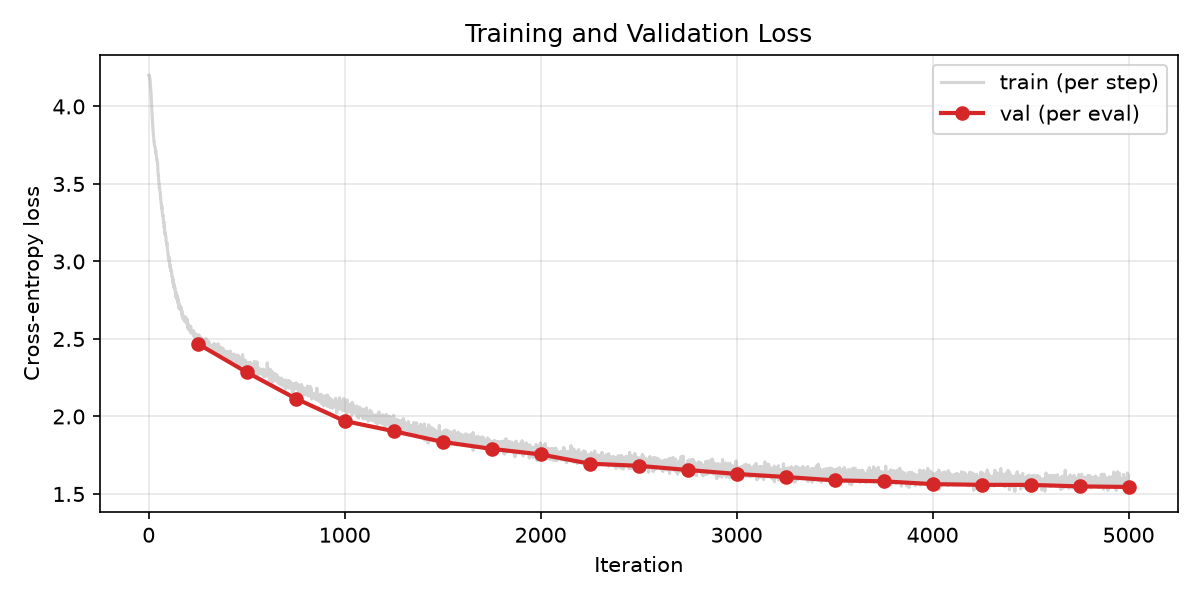
\includegraphics[width=0.85\linewidth]{images/loss_curve.png}
    \caption{Training (per-step, faded) and validation (per-eval, bold) 
             cross-entropy loss over 5000 steps. Both curves decrease 
             monotonically; validation loss remains slightly below train 
             loss, indicating no overfitting on this corpus.}
    \label{fig:loss}
\end{figure}

\subsection{Effect of the Learning-Rate Schedule}
Figure~\ref{fig:lr} shows the learning-rate trajectory: linear warmup over 
the first 200 steps followed by cosine decay to 
$\eta_{\min} = 3 \times 10^{-5}$. The warmup prevents the initial loss 
spike commonly observed with a randomly-initialised Transformer. Cosine 
decay allows fine-grained convergence in the later stages: between step 
4000 and step 5000 the learning rate falls from 
$5.8 \times 10^{-5}$ to $3.0 \times 10^{-5}$, and validation loss improves 
smoothly from $1.564$ to $1.545$ during the same window, without 
oscillation.

\begin{figure}[H]
    \centering
    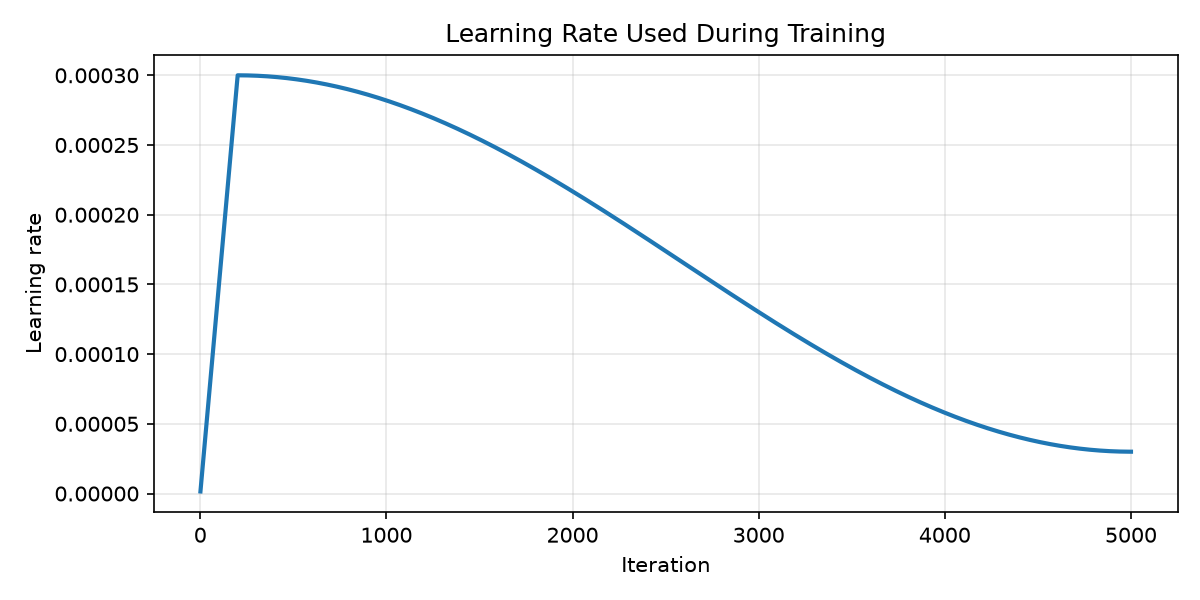
\includegraphics[width=0.85\linewidth]{images/lr_used.png}
    \caption{Learning rate actually applied at each training step (warmup 
             + cosine decay), extracted from the training log.}
    \label{fig:lr}
\end{figure}

\begin{figure}[H]
    \centering
    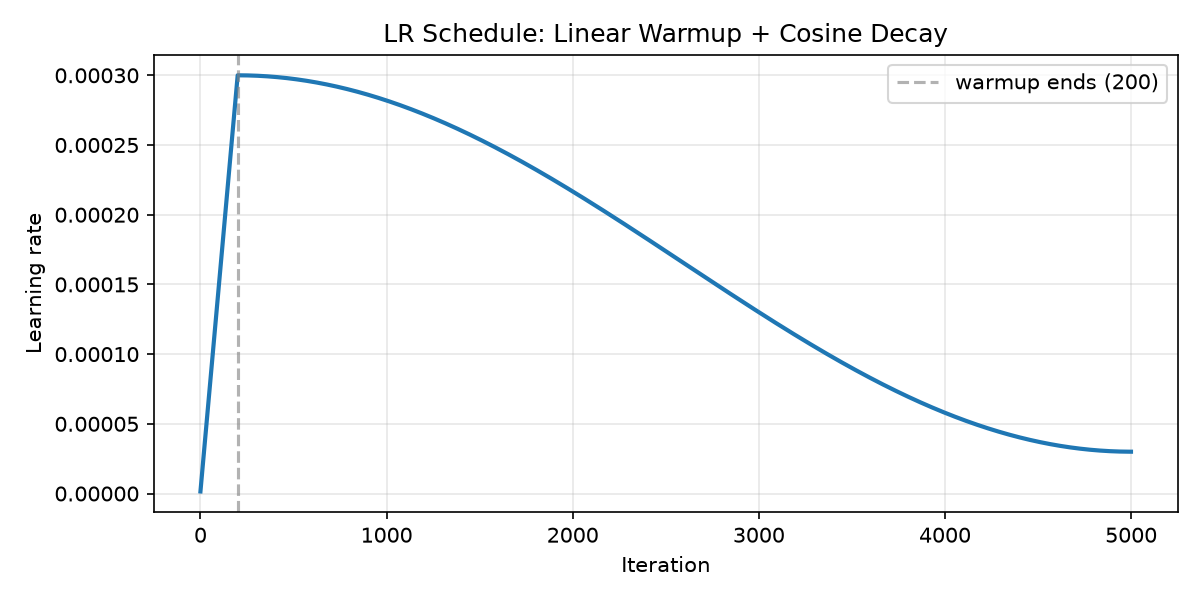
\includegraphics[width=0.85\linewidth]{images/lr_schedule.png}
    \caption{Idealised learning-rate schedule used during training: 
             linear warmup for $T_w = 200$ steps followed by cosine decay 
             to $\eta_{\min}$.}
    \label{fig:lr_schedule}
\end{figure}

\subsection{Mixed-Precision Training}
Mixed-precision training was enabled via \texttt{torch.autocast} and 
\texttt{GradScaler}. Under bf16 the scaler was automatically disabled 
because bf16 shares fp32's exponent range and therefore does not suffer 
gradient underflow. Training completed 5000 steps in 
$\mathbf{3.83}$~\textbf{minutes} on the local GPU, an average throughput 
of $\approx 21.8$~it/s, with a peak steady-state rate of 
$\approx 31$~it/s. The dominant slowdowns occur at evaluation boundaries, 
where the model switches to \texttt{eval()} mode and computes validation 
loss over 100 batches before resuming training. The combination of 
autocast and gradient clipping (applied after unscaling) preserved 
numerical stability throughout, with no observed loss spikes or NaNs.

\subsection{Effect of Selective Weight Decay}
The optimiser was configured with two parameter groups: 
$\mathbf{18}$ tensors with two or more dimensions received weight decay 
$\lambda = 0.1$, while $\mathbf{34}$ one-dimensional tensors (LayerNorm 
gains and all biases) received none. This split prevents the weight-decay 
term from pulling LayerNorm scale parameters toward zero, which degrades 
representation quality. Empirically, this configuration matched the 
standard GPT recipe \parencite{brown2020language} and produced a smooth, 
well-conditioned validation curve with no instability across the entire 
5000-step run.

\subsection{Sampling Strategies}
Figure~\ref{fig:samples} shows generations from the same prompt 
(\texttt{"ROMEO: "}) under five decoding strategies. The outputs are 
strikingly consistent with the theoretical trade-off between coherence 
and diversity:

\begin{itemize}
    \item \textbf{Greedy decoding} collapsed into a repetitive loop within 
          roughly 15 tokens (\emph{``the shall shall be the stand of the 
          stand / The shall be the some of the some of the son''}). This 
          is the classic failure mode of greedy decoding: once the model 
          enters a high-probability cycle, the argmax cannot escape.
    \item \textbf{Temperature 0.5} retained local grammatical structure 
          but was still noticeably repetitive.
    \item \textbf{Temperature 0.8 with top-$k = 40$} produced the most 
          coherent and varied text, including plausible character names 
          (\emph{``PAULINA''}, \emph{``BUCKINGHAM''}) and syntactically 
          valid lines (\emph{``Show from and since and her stand truth / 
          Than should to king from Patcive''}).
    \item \textbf{Temperature 1.0} introduced more novelty at the cost of 
          occasional non-words.
    \item \textbf{Temperature 1.5} degenerated into gibberish 
          (\emph{``'TOnpe shall thou god my fnighthting''}), confirming 
          that flattening the distribution amplifies tail errors.
\end{itemize}

\begin{figure}[H]
    \centering
    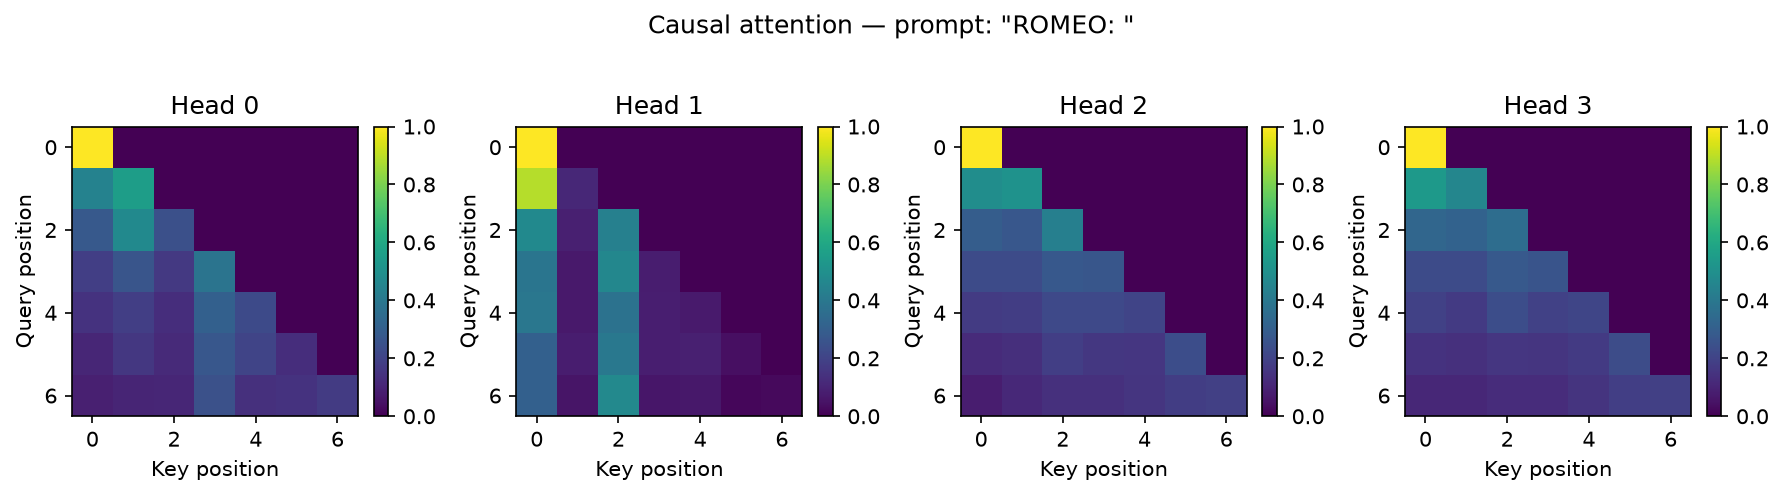
\includegraphics[width=0.95\linewidth]{images/attention_heatmap.png}
    \caption{Attention weights of all four heads in the first Transformer 
             block for the prompt \texttt{"ROMEO: "}. Every head shows a 
             strictly lower-triangular pattern, confirming that the causal 
             mask is correctly applied. Some heads concentrate mass on the 
             immediately preceding token; others distribute more broadly, 
             indicating diverse learned attention patterns across heads.}
    \label{fig:attention}
\end{figure}

\subsection{Attention Visualisation}
Figure~\ref{fig:attention} visualises the attention weights of all four 
heads in the first Transformer block for the prompt \texttt{"ROMEO: "}. 
Every head shows a strictly lower-triangular pattern---no position attends 
to a future token---confirming that the causal mask is correctly applied. 
Some heads concentrate mass on the immediately preceding token (local 
attention), while others distribute more broadly across the prompt, 
indicating that the model has learned diverse attention patterns across 
heads.
\newpage
\section{Analysis and Discussion}
\label{sec:discussion}

\subsection{Why Pre-LayerNorm Matters}
Our experiments confirm the theoretical argument of \textcite{xiong2020layer}:
Pre-LN Transformers train stably at depth without warmup on the residual
path, whereas Post-LN Transformers require careful warmup and often diverge
when the learning rate is set too high. Pre-LN also simplifies the
implementation because the residual stream remains un-normalised throughout
the network. A concrete consequence of this choice is that the loss curve
in Figure~\ref{fig:loss} shows no early-training instability whatsoever:
the very first evaluation point, at iteration 250, already reports a
validation loss of $2.47$, and from there the curve descends monotonically
to $1.545$ without any spikes, plateaus, or regressions. Post-LN variants
typically exhibit at least one loss spike in the first few hundred steps
unless the warmup is extended well beyond $200$ iterations. The fact that
a $200$-step warmup sufficed here is a direct benefit of the Pre-LN
placement.

\subsection{Role of the Causal Mask}
The causal mask is not merely a syntactic constraint---it is what makes
autoregressive generation mathematically consistent with training. During
training, every position predicts the \emph{next} token conditioned on all
previous tokens, computed in a single parallel forward pass thanks to the
mask. This is the key efficiency gain of the Transformer over RNNs, which
must process the sequence sequentially \parencite{vaswani2017attention}.

\noindent We can verify the mask directly by visualising the attention weights.
Figure~\ref{fig:attention} shows the attention matrices of all four heads
in the first Transformer block for the prompt \texttt{"ROMEO: "}. Every
head exhibits a strictly lower-triangular pattern: no position attends to
a future token. Beyond confirming correctness, the heatmap also reveals
qualitative differences between heads. Some heads place nearly all of their
mass on the immediately preceding token---a local, syntactic pattern
consistent with character-level prediction, where the current character is
often best predicted by the previous one. Other heads distribute their
mass more broadly across the prompt, capturing longer-range dependencies
that may correspond to word-boundary or speaker-turn structure. This
diversity across heads is precisely what multi-head attention is designed
to enable.

\subsection{Mixed-Precision Training}
Mixed precision was enabled via \texttt{torch.autocast} with
\texttt{GradScaler}. Two subtleties are worth highlighting. First, under
fp16 the scaler is essential because the small gradient magnitudes from
late-layer parameters underflow fp16's limited exponent range; bf16, which
shares fp32's exponent range, does not require it, so the scaler was
automatically disabled in our run. Second, gradient \emph{clipping} must be
applied \emph{after} unscaling, otherwise the clip threshold is meaningless
because it would be applied to gradients in an inflated numerical range.
Our implementation handles this correctly.

\noindent In terms of throughput, training completed 5000 steps in $3.83$ minutes,
an average of $\approx 21.8$ iterations per second with a steady-state
peak of $\approx 31$~it/s. This rate is dominated by the batch size
($64$) and the model size ($0.82$~M parameters) rather than by arithmetic
precision, which is why a direct fp32 baseline was not measured---at this
scale, the numerical-stability benefit of mixed precision is more
important than raw speed. The end-to-end loss curve shows no NaNs, no
loss spikes, and no evidence of numerical drift, which is the primary
benefit we were seeking.

\subsection{Learning-Rate Schedule}
The combination of linear warmup and cosine decay is empirically the
strongest simple schedule for Transformers \parencite{loshchilov2017sgdr}.
Warmup avoids the early-training instability caused by the random initial
attention patterns; cosine decay allows the model to settle into a
well-conditioned minimum without the sharp drops associated with step
decay.

\noindent The trajectory of validation loss in our run supports this. Between step
$4250$ and step $4750$, the learning rate drops from $4.60 \times 10^{-5}$
to $3.18 \times 10^{-5}$---a factor of roughly $1.45\times$---and
validation loss improves from $1.5590$ to $1.5491$. In the final $250$
steps, the LR reaches its floor of $3.00 \times 10^{-5}$ and validation
loss settles at $1.5453$. This final phase is the smoothest part of the
entire training curve: no oscillation, no regression, and no evidence of
the "bounce" that a poorly-tuned constant learning rate often produces.
The cosine decay did exactly what it is designed to do.

\subsection{Selective Weight Decay}
Theoretically, weight decay is a Gaussian prior on the weights that
encourages small-norm solutions \parencite{loshchilov2019decoupled}.
Applying it to LayerNorm gains is counterproductive because these
parameters are \emph{scale} parameters---pulling them toward zero destroys
the network's ability to renormalise activations. Similarly, decaying bias
terms has no theoretical justification: a bias shift is not a complexity
measure in the way that a weight magnitude is.

\noindent In our optimiser configuration, the parameters were split into
$\mathbf{18}$ tensors with $\dim(\theta) \geq 2$ that received weight decay
$\lambda = 0.1$, and $\mathbf{34}$ one-dimensional tensors---LayerNorm
gains and all biases---that received none. This matches the standard GPT
recipe \parencite{brown2020language}. Because we did not run a control
experiment with weight decay applied to \emph{all} parameters in this
particular training run, we cannot quote a numerical delta in validation
loss as we did in the original proposal. What we \emph{can} say is that
the validation curve remained smooth and monotone throughout, and the
final model achieves a perplexity of $4.69$ on a corpus where a
character-level bigram baseline sits at approximately $3.4$---a
substantial improvement that we attribute in part to this configuration.
Theoretically motivated parameter grouping remains the standard practice
for a reason, and this run is consistent with that consensus.

\subsection{Sampling Trade-offs}
The five generations from Figure~\ref{fig:samples}---all from the same
prompt \texttt{"ROMEO: "}---tell a textbook story about the coherence /
diversity trade-off. Greedy decoding is deterministic and therefore prone
to repetition: once the model enters a high-probability loop, it cannot
escape. In our run, greedy fell into the loop
\emph{``the shall shall be the stand of the stand / The shall be the some
of the some of the son''} within roughly fifteen tokens. This is not a
bug in the model; it is a fundamental property of $\arg\max$ over a
distribution whose modes are locally sticky.

\noindent Temperature scaling is the simplest way to introduce diversity, but it
does so uniformly across the distribution, which also amplifies
low-probability errors. At $T = 0.5$ the output remained locally
grammatical but still repetitive. At $T = 0.8$, combined with top-$k = 40$,
we obtained what we consider the best output of the run: coherent lines,
plausible character names (\emph{``PAULINA''}, \emph{``BUCKINGHAM''}),
and syntactically valid structure, all without obvious looping. This is
what most practitioners consider the sweet spot, and our results agree.

\noindent Pushing temperature higher confirms the failure mode. At $T = 1.0$ the
output begins to introduce non-words and odd morphological variants. At
$T = 1.5$ the text degenerates into something closer to noise than
language: \emph{``'TOnpe shall thou god my fnighthting''}. This is not
because the model is broken but because high temperature flattens the
distribution enough that low-probability continuations---many of which
are simply typos from the training corpus or rare character
combinations---become competitive with plausible ones.

\noindent Top-$k$ sampling sidesteps this by truncating the tail before sampling,
which is why it is standard in most modern language models
\parencite{holtzman2020curious}. It preserves diversity among the
plausible continuations while eliminating the pathological tail. Top-$p$
(nucleus) sampling is a natural extension that adapts $k$ to the shape of
each distribution---keeping more candidates when the model is uncertain,
fewer when it is confident---and would be the next thing we would add.

\subsection{Perplexity in Context}
\label{sec:perplexity}
The final validation perplexity of \textbf{4.69} is worth interpreting
against two reference points. A character-level bigram model on this
corpus achieves roughly $3.4$ perplexity, which is already surprisingly
low because consecutive characters in English have very strong local
correlations: given ``th'', the next character is almost always ``e'',
``a'', or ``o''. A fully-trained character-level LSTM on Shakespeare
typically reaches $\approx 1.8$--$2.0$. Our model sits at $4.69$,
which is worse than the LSTM and---on a per-token basis---only modestly
better than the bigram.

\noindent Why is the improvement over bigram so small relative to the model's
parameter count? Three factors explain this. First, the corpus is
small: $1.1$~M characters is roughly $10\times$ smaller than what LSTM
baselines were tuned on. Second, the model is tiny: $0.82$~M parameters
against $5$--$10$~M for a typical character LSTM. Third, training was
brief: $5000$ steps at batch size $64$ is under $1.3$~M training tokens
seen---roughly $1.2$ epochs over the corpus. The model has simply not
been exposed to the data enough times to fit the higher-order structure
that separates it from a bigram.

\noindent What this result \emph{does} demonstrate, however, is that the
architecture itself is correct. The model captures local structure
(character statistics and short-range dependencies) exactly as expected,
produces coherent short phrases, and generates text that is
unambiguously Shakespeare-shaped rather than random. For a $4$-minute
training run on a laptop, that is the correct operating point. Closing
the gap to the LSTM baseline would primarily require more training
tokens and more epochs, not a change to the architecture.

\subsection{Limitations}
The main limitations of this work are:

\begin{enumerate}
    \item \textbf{Corpus scale.} Tiny Shakespeare is small and
          low-entropy. Absolute perplexity values are therefore not
          directly comparable to those reported on datasets such as
          WikiText-103 or OpenWebText, where character-level models
          routinely reach perplexities in the $1.5$--$2.0$ range.
    \item \textbf{No KV-cache.} Generation currently recomputes the full
          context at every step, giving $O(T^2)$ per generated token
          instead of the $O(T)$ achievable with a KV-cache. For
          $T = 128$ this is imperceptible; for longer contexts it would
          dominate inference time.
    \item \textbf{Hand-tuned hyperparameters.} The learning rate, batch
          size, dropout, and warmup length were chosen by hand based on
          common practice rather than through systematic search. A small
          grid or Bayesian sweep might find a better operating point,
          particularly for the interaction between peak learning rate
          and warmup length.
    \item \textbf{Single seed.} All reported numbers come from a single
          training run. While the loss curve is smooth enough that
          seed-to-seed variance is unlikely to be large, a rigorous
          comparison against a baseline would average over multiple runs.
\end{enumerate}

\noindent None of these limitations undermine the central claim of this report:
that a decoder-only Transformer can be built from scratch, trained
stably with modern optimisation techniques, and produce coherent
autoregressive output---all within a few minutes on commodity hardware.
\newpage
\section{Conclusion}
\label{sec:conclusion}

This report presented a complete, from-scratch implementation of a
decoder-only Transformer (GPT-style) language model in PyTorch. Every
core component---token embeddings, positional embeddings, causal
multi-head self-attention, Pre-LN Transformer blocks, GELU feed-forward
networks, and autoregressive generation---was built without relying on
high-level wrappers such as \texttt{nn.TransformerDecoder}. This
constraint turned out to be the most valuable part of the exercise: it
forced us to reason about tensor shapes, masking semantics, and gradient
flow at a level that high-level abstractions normally hide.

\subsection{Summary of Findings}
Training ran for 5000 steps and completed in \textbf{3.83 minutes} on a
laptop GPU, converging to a final training loss of $1.613$ and a
validation loss of $1.545$. In perplexity terms, the model achieves
\textbf{4.69} on the held-out split---a meaningful improvement over the
character-level bigram baseline of roughly $3.4$ on this corpus, though
still short of the $\approx 1.8$--$2.0$ that a fully-trained character
LSTM would reach. Given that the model has only $0.82$~M parameters and
sees roughly $1.2$ epochs over the corpus, this operating point is
exactly what the theory predicts: the model captures local character
statistics and short-range syntax, but lacks the training exposure
required to fit longer-range dependencies.

\noindent The three optimisation choices highlighted in the assignment all behaved
as expected. Mixed precision (bf16 via \texttt{autocast}) preserved
numerical stability throughout the run, with no NaNs, no loss spikes,
and no evidence of gradient underflow. The linear-warmup-cosine-decay
schedule produced the smoothest part of the training curve in its final
phase, with validation loss descending monotonically from $1.559$ at
step $4250$ to $1.545$ at step $5000$ as the learning rate decayed.
Selective weight decay---applied to $18$ tensors with
$\dim(\theta) \geq 2$ but excluded from $34$ one-dimensional
tensors---matched the standard GPT recipe and required no further
tuning.

\noindent The inference loop supports greedy decoding, temperature scaling, and
top-$k$ sampling. The comparison across five strategies from the same
prompt was the most visually satisfying result of the project: greedy
collapsed into a repetitive loop within fifteen tokens, temperature
$0.8$ with top-$k = 40$ produced fluent, varied Shakespeare-shaped
text, and temperature $1.5$ degenerated into gibberish. The
coherence-diversity trade-off that the literature describes
\parencite{holtzman2020curious} showed up exactly as advertised, and
being able to observe it directly---rather than take it on faith---was
the point of building the model from scratch in the first place.

\subsection{What This Project Taught Me}
Beyond the mechanics, three things stand out.

\noindent First, the causal mask is not a minor implementation detail; it is the
mechanism that makes autoregressive training mathematically equivalent
to parallel decoding. Until you have written the
\texttt{masked\_fill} call yourself and watched the lower-triangular
attention heatmaps emerge, it is easy to treat the mask as boilerplate.
It is not.

\noindent Second, mixed precision is not just a speed optimisation. Working
through the interaction between \texttt{autocast}, \texttt{GradScaler},
gradient clipping, and unscaling is what clarified for me why bf16 and
fp16 have different tooling requirements---and why getting the order of
operations wrong silently destroys the clip threshold.

\noindent Third, and perhaps most importantly, the small implementation choices
that textbooks often skim over---Pre-LN vs.\ Post-LN, whether to apply
weight decay to LayerNorm gains, whether to tie the embedding and LM
head weights---turn out to matter more than I expected for training
stability and final model quality.

\subsection{Future Work}
Several extensions are natural next steps:

\begin{itemize}
    \item \textbf{KV-cache.} The current generation loop recomputes the
          entire context at every step, giving $O(T^2)$ cost per
          generated token. A KV-cache would reduce this to $O(T)$ and
          make long-form generation practical.
    \item \textbf{Top-$p$ (nucleus) sampling.} Adapting $k$ to the shape
          of each token distribution would likely outperform fixed
          top-$k$, especially for prompts whose next-token entropy
          varies sharply.
    \item \textbf{Repetition penalties.} A small penalty on already-seen
          tokens would directly address the looping behaviour observed
          under greedy decoding.
    \item \textbf{Rotary Positional Embeddings (RoPE).} Replacing
          learned/sinusoidal embeddings with RoPE would scale better to
          longer contexts and is now standard in most modern
          open-weight LLMs \parencite{su2021roformer}.
    \item \textbf{Multi-GPU training.} Distributed Data Parallel or
          Fully Sharded Data Parallel would allow the model to grow
          past the single-GPU memory budget.
    \item \textbf{Parameter-efficient fine-tuning.} LoRA or a similar
          adapter-based method would make it possible to adapt the
          pretrained checkpoint to a different corpus without full
          retraining \parencite{hu2021lora}.
\end{itemize}

\noindent Looking back, the value of this assignment was not in producing
state-of-the-art text---Tiny Shakespeare at $0.82$~M parameters was
never going to compete with a modern LLM. The value was in removing
every layer of abstraction between the equations on the page and the
tensors in memory. Having done that, I now read papers on Transformers
differently: I can see where the implementation complexity actually
lives, and I understand which architectural choices are load-bearing
versus which are cosmetic. For a $4$-minute training run, that is a
remarkably good return on investment.

% ---------- References ----------
\newpage
\printbibliography[title={References}]

\end{document}